%----------------------------------------------------------------------------------------
%   PACKAGES AND OTHER DOCUMENT CONFIGURATIONS
%----------------------------------------------------------------------------------------

\documentclass[11pt]{article}

\usepackage[english]{babel}
\usepackage[utf8x]{inputenc}
\usepackage{amsmath}
\usepackage{graphicx}
\usepackage{csquotes}
\usepackage{fancyvrb}
\usepackage[a4paper, total={6in, 8in}]{geometry}
\usepackage[colorinlistoftodos]{todonotes}

%----------------------------------------------------------------------------------------
%   HEADING
%----------------------------------------------------------------------------------------

\newcommand{\BigO}[1]{\ensuremath{\operatorname{O}\left(#1\right)}}

\title{\textsc{Software Engineering}\\Main Coursework II}
\author{Lawrence Jones \{lmj112\} \  Alice Sibold \{as4712\} \\
        Joshua Coutinho \{jrc12\}}

\date{}
\begin{document}
\maketitle

%----------------------------------------------------------------------------------------
%   BODY
%----------------------------------------------------------------------------------------

GoCardless is a FinTech startup based in Angel, London. They provide an API that
instruments DirectDebit payment networks to pull money between bank accounts,
and have been doing so since 2011. Their main product is their API, making
GoCardless a great case study for development practises in modern technological
start-ups.

In contrast, Amazon is the largest internet retailer in the United States with
an internationally recognised brand. Launched over two decades ago (1994) Amazon
stands as one of the greatest successes of the internet age, having weathered
the dot-com collapse (2000) and outlasted a long list of direct competitors.
Amazon also happens to support one of the worlds largest micro-service
architectures after hitting a hard barrier in 2001, when its C++ Obidos monolith
would take over a weekend to compile.

This article aims to compare how the software development lifecycle (SDLC)
differs between two companies with disparate operational scales, company history
and ethos. Techniques that work well for one company can become severe
hindrances when scaled, and it will be interesting to see which survive over
the course of that transformation.

\section{Conception}

Developers at GC tackle new features with a `kick off' meeting, consisting of
the core development team working on the feature and any other essentially
involved people from around the company. The aim is to discuss the critical (or
happy) path of the feature, describing the experience for the standard user.
During this process any issues can be raised while the people with domain
knowledge are present, allowing the plan to adjust to immediate feedback before
any real work is done.

Over the next couple of days the team of developers will produce a `scoping
document' (Figure~\ref{fig:scoping}), detailing their implementation plan
and capturing the results of research around the feature. This document is
usually written in some sort of collaborative environment (Google Docs, Dropbox
Paper, etc.) with a link being shared directly to anyone involved in the
project, and made available to entire company.

\begin{figure}
\centering
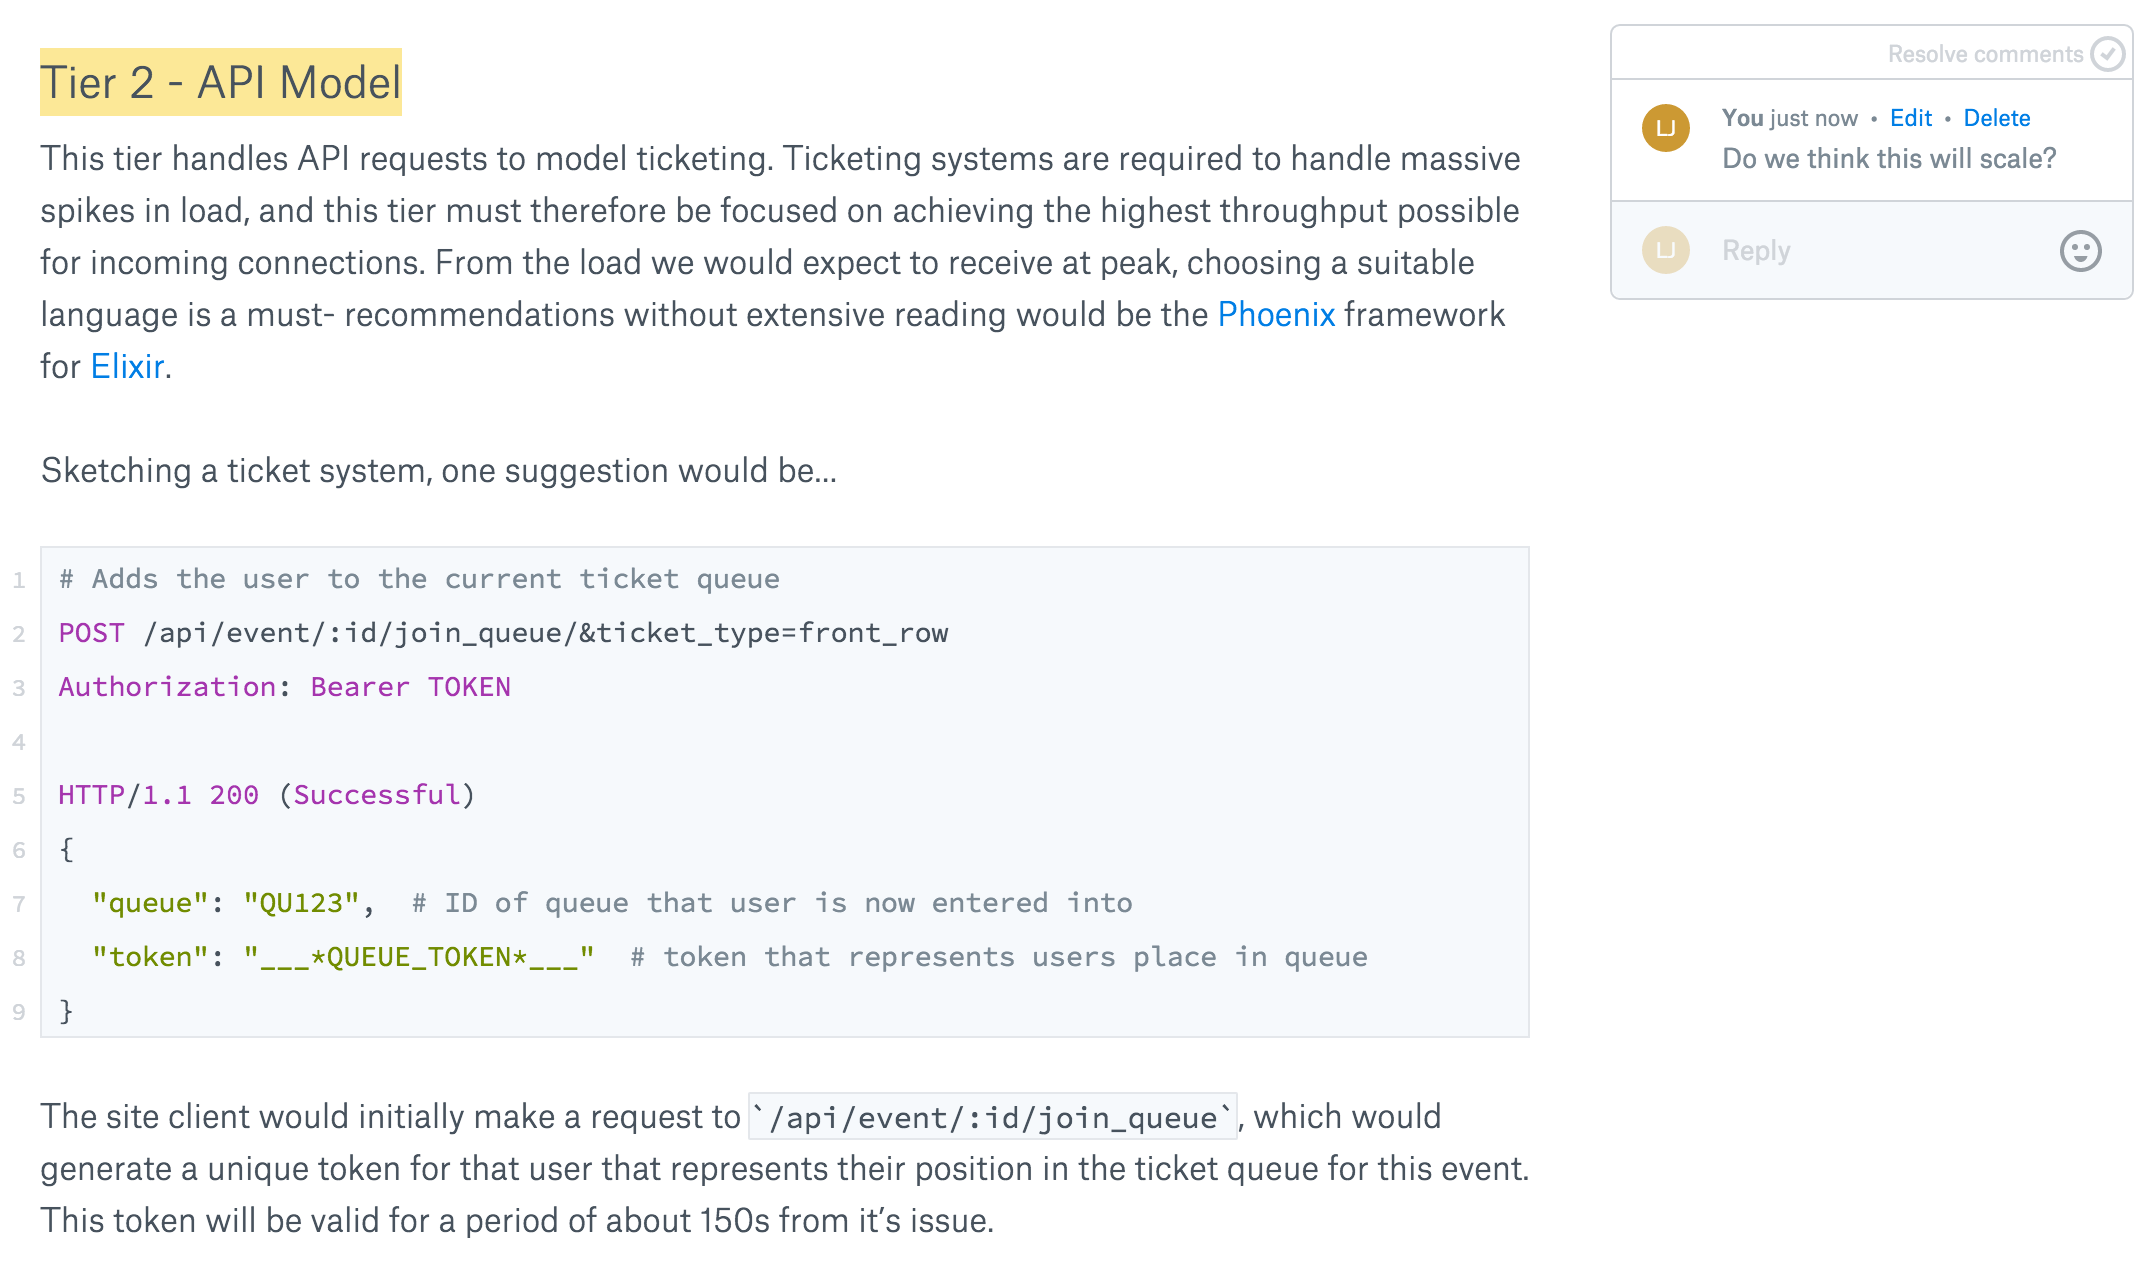
\includegraphics[width=0.9\textwidth]{lib/res/scoping.png}
\caption{\label{fig:scoping}\textit{Example scoping document- mix of technical with
free-form content, including collaborative comments}}
\end{figure}

Working with such visibility enables several operational benefits. Foremost,
rarely does this process produce solutions that differ wildly from the actual
requirements. Developers often lack context when they begin work, so having
others in the company who understand the problem on hand during the design
process means misunderstandings can be easily corrected early, with minimal
cost~\cite{costOfChangeEssay}.

Secondly, opening this document to the entire company increases awareness of
what the development team are working on. For non-developers, this translates
into an understanding of how a large part of the company are spending their
time, and how that work contributes to the overall company's goal. A key
component of any high functioning team is accountability within the
sub-teams~\cite{fiveDysfunctions}, and this only comes when teams have an
understanding of what others are working on.

For developers, this increased visibility means a direct reduction in the
projects bus, or truck factor~\cite{truckFactor}. When other developers can share
in the design process they learn crucial information that will help them
troubleshoot this code when problems arise in the future. On top of this, any
developers who conceive an alternative approach or predict problems with the
design have a clear forum for discussion.

At Amazon new employees are told it matters little who makes business proposals,
so long as the proposal is grounded in solid research. The preferred method of
raising communication between teams are whitepapers, a type of summary document
written in free-form with effort made for concision. The motivation behind this
medium is to force the presenter to compact their research into its most
essential form, producing an easily digestible document that can serve as a base
for further research in the area.

Amazon's whitepapers are very similar in content to GoCardless's scoping
document, and have much the same aim even when a whitepaper lacks the
collaboration encouraged by online tools. Each aims to be concise and follow a
top down structure~\cite{reportingAndWriting}, where each subsequent section
talks at an increasing level of detail. This aids inter-team communication and
allows at least part of the documents to be readable with varying levels of
technical expertise, while providing space for highly technical detail if
required.

The effect of considered writing on designing software is profound. The
requirement of precision in the writing forces the developer to identify
assumptions behind each stage of the project plan, bringing bad assumptions into
harsh relief. By walking through each step of the implementation the developer
naturally questions what each task will consist of, cultivating an awareness
that leads to an improvement in estimation accuracy and a reduction in surprises
during the implementation.

The Agile Manifesto~\cite{agileManifesto} states “[We value] working software
over comprehensive documentation” which has impacted the perceived value of an
up-front technical document to many modern developers. We argue that a scoping
document or whitepaper does not constitute “comprehensive” documentation, and
that the advantages of writing such a document are as relevant now as when Joel
Spolsky wrote his article “Painless Functional Specifications - Why Bother?” in
2000.

Joel argues that technical documents (`specs') can provide a tool to funnel out
inaccurate assumptions developers may have about the product, before they write
the inaccurate code. We tackle this problem at the earliest stage, before our
software resembles “a compromise between the initial, wrong design and the ideal
design”. This focus also lends itself to forcing decisions on the hardest
problems, those which are often put off until the last moment, despite being the
issues most likely to cause a software project to fail.

Technical documents may be considered by some as heavyweight tools, long since
replaced in software engineering. We counter that they remain a valuable tool to
aid developer investigation into a problem, as well as an anchor for inter-team
communication. That Amazon and GoCardless both use such tools, representing
fast-moving environments striving for optimal efficiency, suggests that
technical writing may be less restrictive than it at first seems.

\section{Testing \& Continuous Delivery}

Amazon recently released tools that allow developers to automate code deployment
to AWS machines via the AWS console. Specifically, the two tools AWS CodeDeploy
and CodePipeline are continuous delivery instruments, and bring advanced
deployment tools within reach of your standard developer.

\begin{figure}
\centering
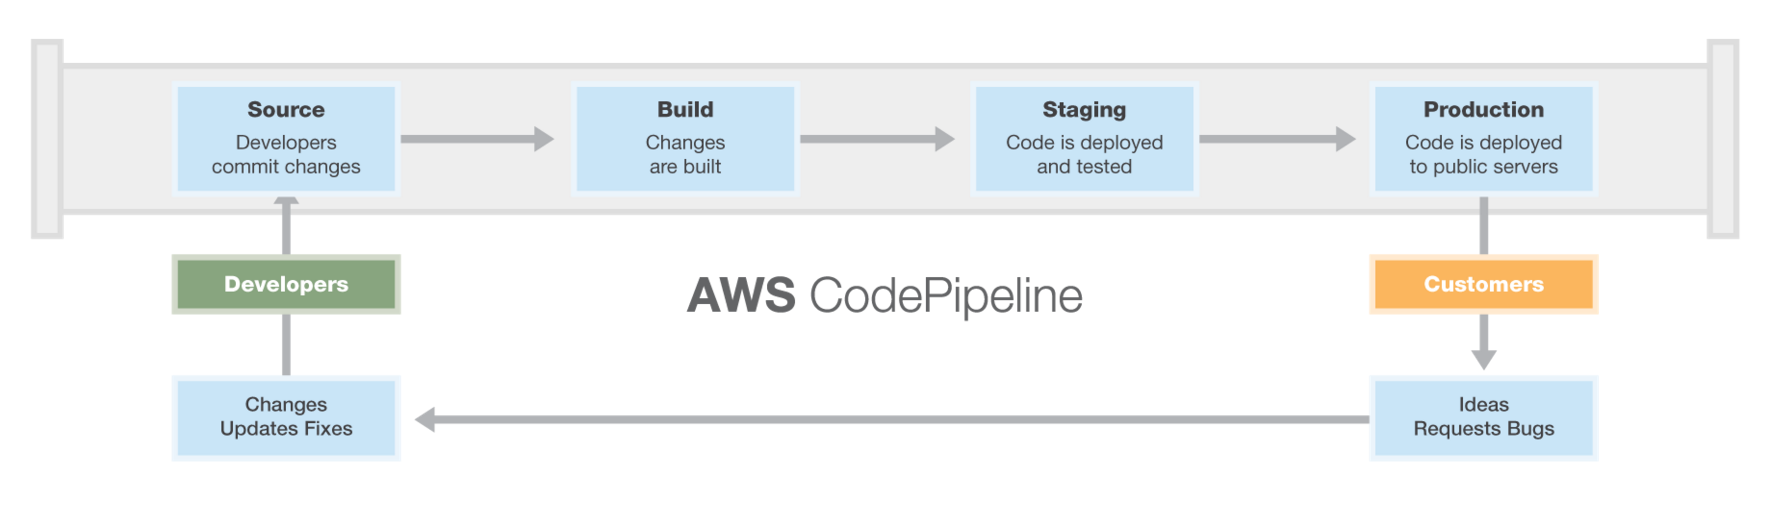
\includegraphics[width=0.8\textwidth]{lib/res/code_pipeline.png}
\caption{\label{fig:scoping}\textit{Diagram from Amazon webpage on
CodePipeline}}
\end{figure}

While this is the first time tools like this have been offered by Amazon
commercially, the business has been making use of internal tools for these
purposes for many years. Amazon's platform is built on top of micro-services;
whenever anyone visits an Amazon webpage up to 150 services are invoked for the
page render. As one of the first companies to embrace micro-services, Amazon
tackled novel growing pains as they built out their architecture from the old
monolith.

One of the most pressing of these pains was how much developer time was sunk
into deployments. Now Amazon was split into many services, each team had settled
on a slightly different deployment strategy. When deployment means
\texttt{ssh}'ing into a single box, this might not cause too much frustration,
but Amazon teams were looking to deploy to fleets of hundreds of servers with
zero-downtime requirements. Lacking a unified toolchain for deployments meant
each team would spend a large amount of time re-inventing the wheel, producing a
bespoke deployment process for their service. Werner Vogels describes the
problem\dots

\begin{displayquote}

  Each team took on full ownership of the development and operation of a single
  service\dots teams were able to quickly produce new features, but their deployment
  process soon became a bottleneck. Manual deployment steps slowed down releases
  and introduced bugs caused by human error. Many teams started to fully
  automate their deployments to fix this, but that was not as simple as it first
  appeared.

  \textit{Excerpt From: The Story of Apollo - Amazon's Deployment
  Engine~\cite{theStoryOfApollo}}

\end{displayquote}

These problems led directly to the creation of Amazon's internal deployment
platform, Apollo, or as it is now known, CodeDeploy. `The Deployment Production
Line'~\cite{deploymentProductionLine} states some qualities that a good
deployment system should demonstrate, and Apollo solved many of these.

The first is automating deployments. One of the biggest advantages Apollo could
offer was full, intelligent automated deployment of services, across a fleet of
AWS servers. Once configured, Apollo could deploy code to any required
environment, spinning up servers to match the application's scaling profile, and
configuration changes could be made on the fly without taking down the service.
This capability was far beyond any of the custom shell scripts teams had written
to deploy their apps, as Apollo benefitted from a dedicated team working full
time on developing its facilities and integrating the tool into Amazon's
infrastructure. This immediately reduced the amount of time developers spent
debugging their deployments.

Humble also states that a deployment tool chain must ensure the same artifacts
are deployed to every environment. Each service at Amazon depends on hundreds of
others, and so building against the correct version-set is essential for
reliability. Amazon solves this problem with another tool, called Brazil, which
is used as the bootstrapper whenever running an Amazon service.

Each service (synonymous here with package) has its own Brazil config file,
which contains a mapping of each dependency to version. Brazil can be used to
pull down and install a service's dependencies but crucially, Brazil can
lockdown a machine to use only those packages installed from the Brazil config.
Each service is invoked through a shim, \texttt{brazil-bootstrap}, which hijacks
the system path to point only to the dependencies installed from the config
file.  All services are built and deployed using Brazil, ensuring that each
environment benefits from repeatable builds that rely on exactly the same
dependency versions.

This method of enforcing good practise on developers is typical of Amazon's
working environment. Having thousands of developers working on Amazon services
precludes simply sending a memo about a new development process; at this scale,
any standard that is not enforced is unenforceable. The power of linking every
developer into a unified deployment tool (such as Apollo) is that company wide
standards can be baked into every teams process.

One of the greatest examples of how Amazon use this power is to enforce a best
practise that almost no one else in the industry has managed to adhere to- unit
tests should run in isolation, without hitting any external resources. Clean
Code~\cite{cleanCode} states five qualities of good unit tests, two of which
demand this property\dots

\begin{displayquote}

  \textbf{Fast}: Tests should be fast. The should run quickly. \\
  \textbf{Repeatable}: Tests should be repeatable in any environment. \\

  \textit{Excerpt From: Robert C. Martin. `Clean Code: A Handbook of Agile
  Software Craftsmanship.'}

\end{displayquote}

When unit tests need to be run fast, they cannot rely upon calling external
components that may take many seconds to generate responses. Repeatability is
also violated when tests depend on external services, as now the test output is
largely dependent on the presence of that service and on whatever result it may
return. While the benefits of writing unit tests in isolation are obvious,
developers typically take this adage as a rule of thumb rather than a hard
limit.

Amazon ensures that all unit tests are written in this fashion by locking down
the boxes that run the unit test pipeline stage. The machines that run unit
tests have firewalls that block any network attempt out, or back into the host,
removing the possibility of communicating with a locally hosted database for
example. Consequently, unit tests for Amazon services typically run in under 10m
including setup and teardown, without relying on any specialised hardware or
parallelisation. This minimises the cost per build while preserving rapid
feedback to developers.

GoCardless has a far more flexible process, encouraged by the use of Ruby on
Rails as the company's stack. Rails uses a framework called
\texttt{ActiveRecord}~\cite{activeRecord} as a database ORM, with many core
Rails features tightly coupled to this interface. \texttt{ActiveRecord}
abstracts away from the underlying database to provide a query interface that
can be called from Ruby code, wrapping the results of each database query in
appropriate Ruby classes.  While this interface provides valuable syntactic
sugar that improves the development experience when interacting with database
records, the coupling of code to \texttt{ActiveRecord} means unit tests
implicitly rely upon an active database connection.

Unit tests that hit \texttt{ActiveRecord} have now broken the `repeatable'
quality that states tests should run in any environment, regardless of
configuration. A standard practise for writing tests in a Rails environment will
make use of gems such as \texttt{FactoryGirl}~\cite{factoryGirl} to create mock
database records before each test run. This practise can be anything but fast,
and without due care test suite running time can balloon dramatically. Writing
tests in this fashion sacrifices some speed and resilience of idiomatic unit
tests, but gains some benefits\dots

\begin{displayquote}

  Writing semi-integration in place of unit tests is just easier than the
  alternative. When the code under test is coupled so tightly with
  \texttt{ActiveRecord} and some of the features like database transactions,
  it's much quicker to not put the work in to build reusable mocks and decompose
  things so they can be tested without hitting the database.

  The trade off is very cheap when the system is small- you don't have many
  tests so even if each one is super-slow it doesn't matter. The problem appears
  when the system grows, as the cost increases exponentially with growth and you
  end up with $>5m$ builds, which can become a waste of developer time. \\

  \textit{Isaac Seymour - Backend developer at GoCardless}

\end{displayquote}

So if this becomes a such a problem, then why are GoCardless willing to suffer it?
\texttt{payments-service}, the core system behind the GoCardless API, is a Rails app
consisting of over 150k lines of Ruby code. Surely this problem should have
crossed the line at which point build times become prohibitively expensive?

Unfortunately, \texttt{payments-service} has a few characteristics that make it
more difficult than your standard Rails app to test in isolation. The first is
due to defensive programming- being a payments service means protecting against
any software error that could cause bad accounting, including race conditions.
GoCardless engineers decided early on to rely on the database layer (in this
instance, PostgreSQL) to provide atomicity guarantees, and so code often relies
on \texttt{ActiveRecord} passing up database exceptions, such as constrint
violations.

Mocking how \texttt{ActiveRecord} handles the underlying database in a unit test
is patently ridiculous. What is meant to be test code tightly focused on the
unit it is testing becomes a game of how well the developer knows
\texttt{ActiveRecord} internals, and is inherently fragile. Mocking a
constraint violations can expose the risk that unit tests will pass (simulating
that constraint being violated) without the constraint ever being encoded into
the database.

When your app moves millions of pounds daily, even that minimal risk cannot be
tolerated. Zach Holman states\dots

\begin{displayquote}

  `We can make good tests run fast but we can't make fast tests be good.'

  So start with a good foundation: have good tests. Don't skimp out on this,
  because it impacts everything else down the line. \\

  \textit{Zach Holman - How to Deploy Software~\cite{howToDeploySoftware}}

\end{displayquote}

Here, GoCardless clearly opted to write good tests over the faster, more brittle
kind they felt were an inevitability had they mocked out the database. But Zach
suggests there is a possibility to push the envelope on how far we can run
with these tests, and indeed GoCardless do just that. By tuning PostgreSQL for
maximal testing performance, you can immediately reduce the running time of
database heavy tests.

While useful, these sort of optimisations only have so much mileage. Zach goes
on to say~\cite{howToDeploySoftware} that test suites should take somewhere in
the range of 5-10m to complete. The simplest way to achieve this is by throwing
more hardware at the problem. The cost of additional infrastructure can be
easily justified in the time it saves for developers when checking in a new
change, and GoCardless tackles this problem by sharding the unit tests across 5
containers when pushing to CircleCI, their CI provider. This brings test suite
running time down to approximately 10m for \texttt{payments-service} as can be
seen in Figure~\ref{fig:circle}, a duration that GoCardless engineers feel is
sufficiently fast.

\begin{figure}
\centering
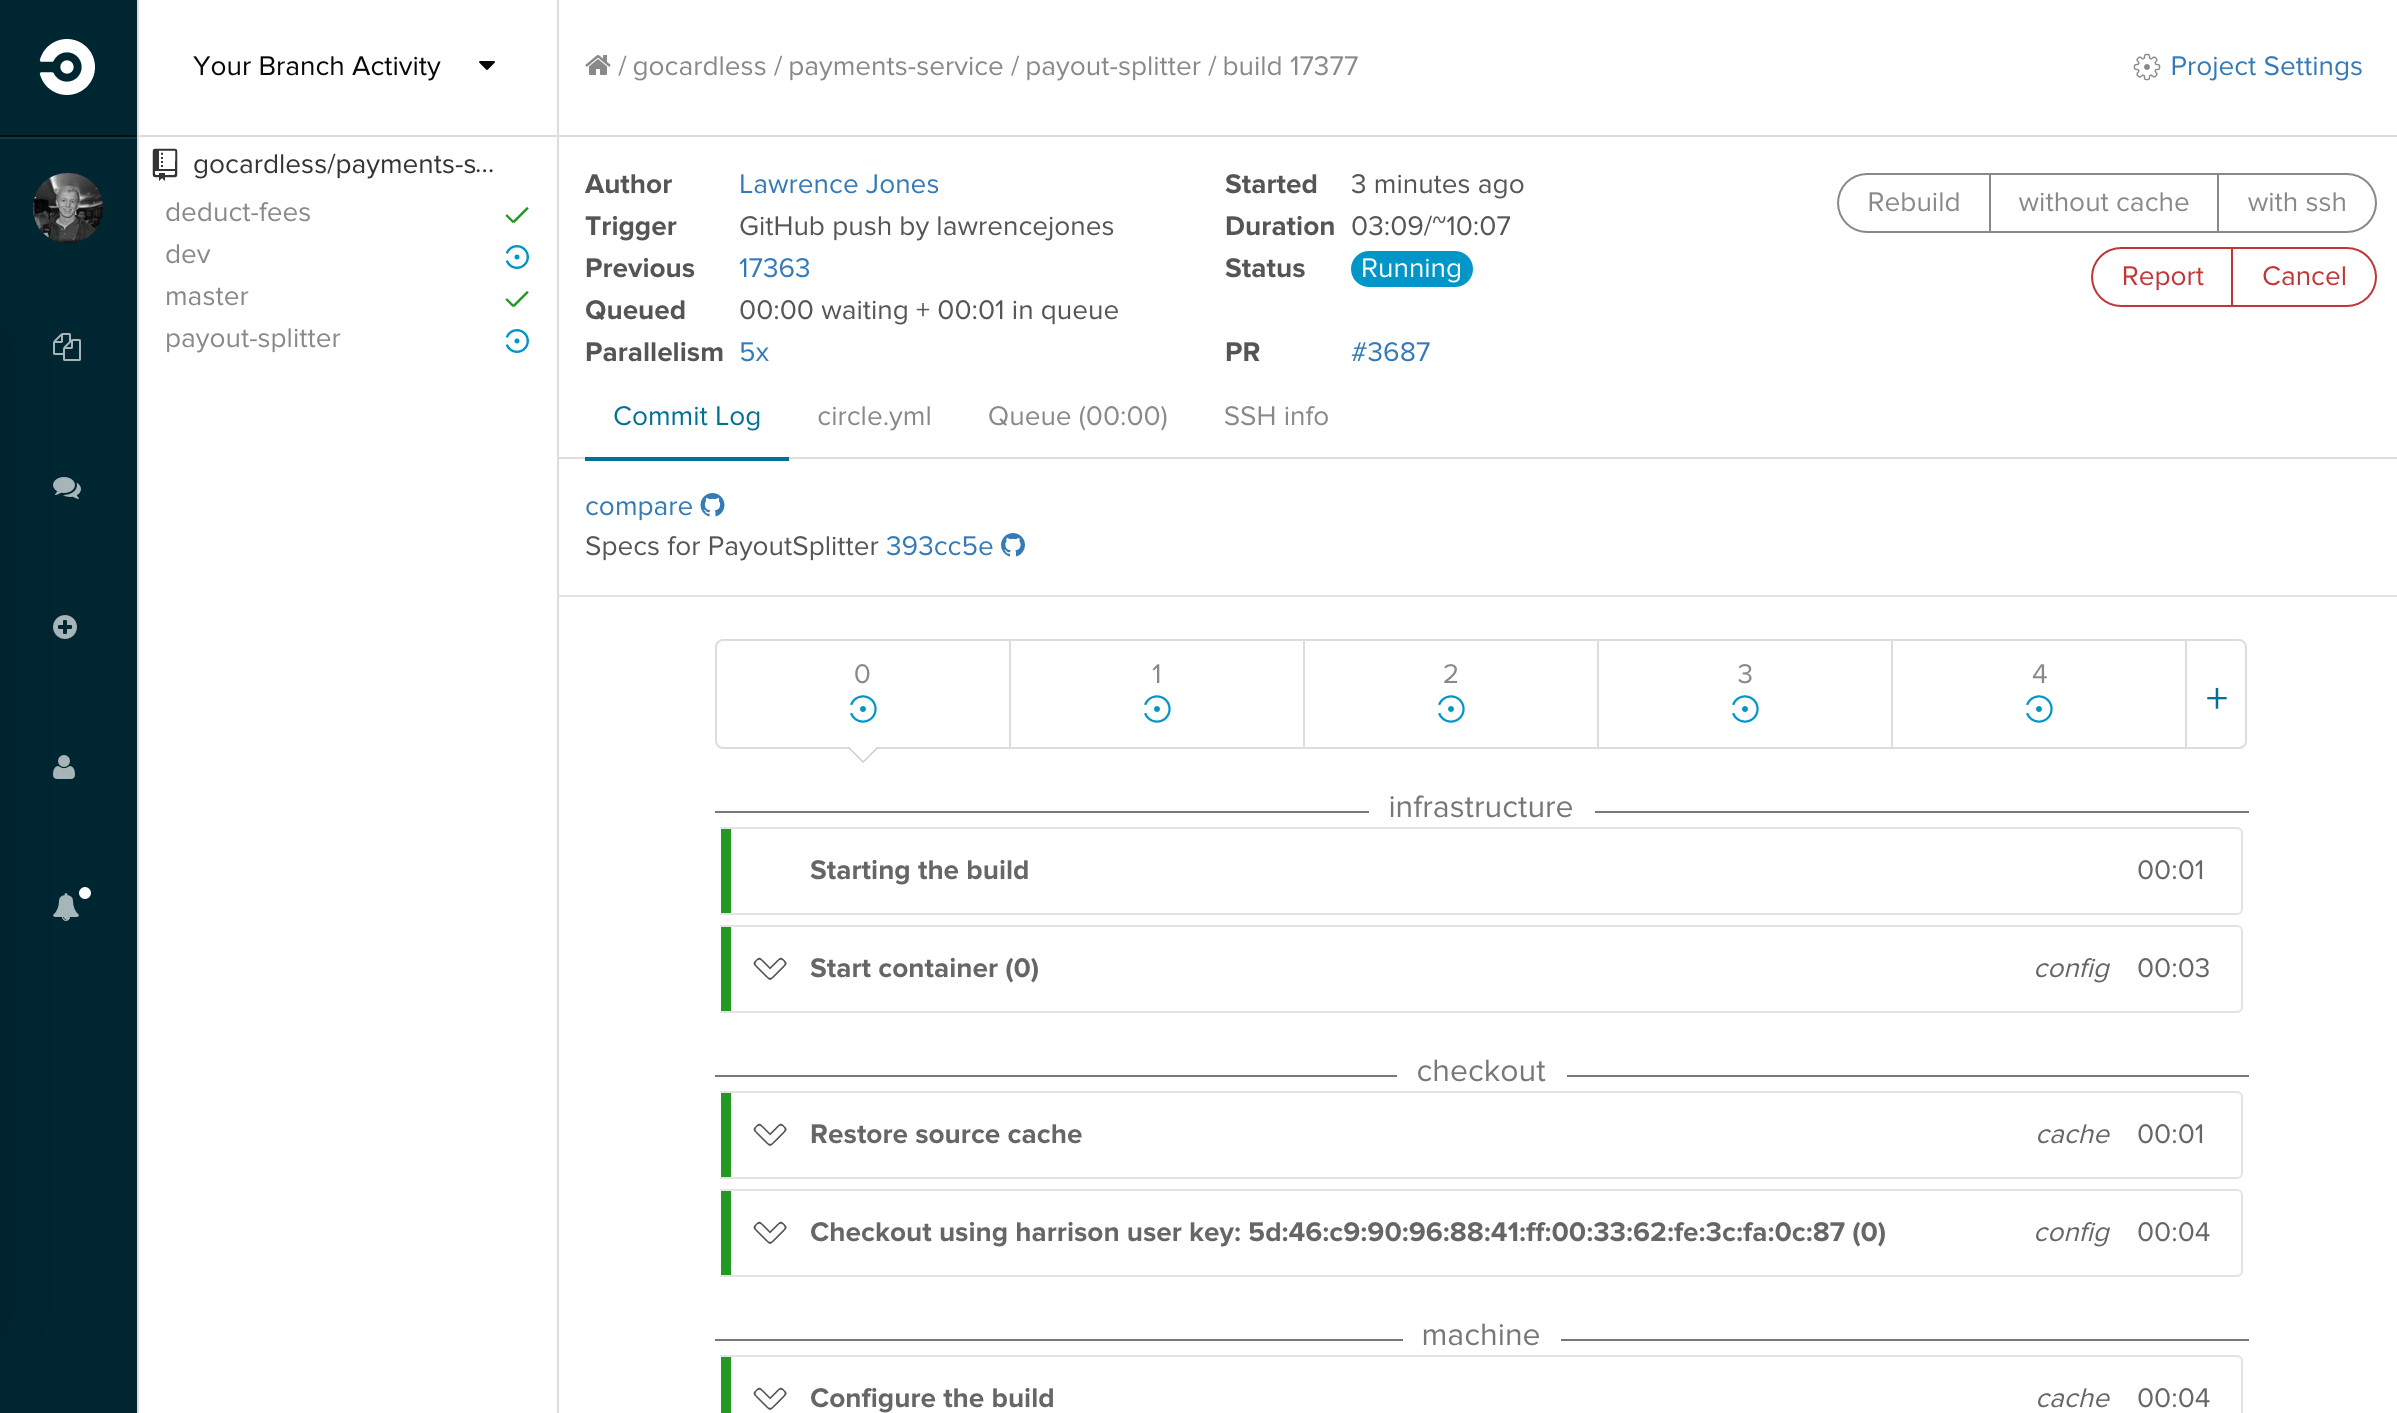
\includegraphics[width=1\textwidth]{lib/res/circle.png}
\caption{\label{fig:circle}\textit{\texttt{payments-service} tests running on
CircleCI with 5 workers}}
\end{figure}

One might ask how far this can scale, and for this Stripe provides an excellent
case study. Built on Rails, just as GoCardless, Stripe have achieved three
minute build times from the natural conclusion of this parallelisation, by
creating their own test runner framework that \texttt{fork}s extensively on a
high powered Amazon EC instance. Stripe's Nelson Elhage says\dots

\begin{displayquote}

  The decision to invest effort in our own testing infrastructure wasn't
  necessarily obvious: we could have continued to use a third-party solution.
  However, spending a comparatively small amount of effort allowed the rest of our
  engineering organization to move significantly faster—and with more confidence.
  I'm also optimistic this test runner will continue to scale with us and support
  our growth for several years to come.\\

  \textit{Nelson Elhage - Running three hours of Ruby tests in under three
  minutes~\cite{stripeDistributedTesting}}

\end{displayquote}

Clearly Stripe figured out how to make their `good tests' run fast, and have
confidence they will continue to do so in future.

\[*\]

The comparison of Amazon and GoCardless testing ethos highlights some major
differences in organisational structure. Amazon with their many services cannot
afford to special case each team, nor as their Frugality principle suggests,
would they want to. GoCardless as a start-up has much more flexibility in this
regard, and can manage each project on its own basis. Indeed, specifying a
general rule for everyone when your company is only four years old is probably
an unwise move.

Regardless of their differences in size and technical ethos, Amazon and
GoCardless both exhibit key qualities of highly effective companies. Both strive
for pragmatism in their development practises, and favour a highly technical
dialogue that works hard to include non-technical staff in the discussion.

Each follow Agile principles, but do so on their own terms. It's highly unusual
to find either adopting a procedure that they haven't questioned the value of
\textbf{within the context of their own business}, which can be refreshing in an
industry that enjoys talking in absolutes.


%----------------------------------------------------------------------------------------
%   BIBLIOGRAPHY
%----------------------------------------------------------------------------------------

\medskip
\bibliography{lib/refs}{}
\bibliographystyle{plain}
\newpage

\end{document}
